\documentclass[a4paper,12pt]{article}

\usepackage[margin=1in,left=1.5in,includefoot]{geometry}
% Graphic
\usepackage{graphicx}
\usepackage{float}

% Hyperlinks
\usepackage{hyperref}

% Header and footer
\usepackage{fancyhdr}
\pagestyle{fancy}
\fancyfoot{}
\fancyhead[LE,RO]{\bfseries\thepage}
\setlength{\headheight}{15pt}

% Quotes character
\usepackage[utf8]{inputenc}

\usepackage{listings}
\lstset{
  basicstyle=\ttfamily,
  columns=fullflexible,
%  frame=single,
  breaklines=true,
  postbreak=\mbox{\textcolor{red}{$\hookrightarrow$}\space},
}

% color links
\usepackage{color}  
\usepackage{hyperref}
\hypersetup{
    colorlinks=true, %set true if you want colored links
    linktoc=all,     %set to all if you want both sections and subsections linked
    linkcolor=black,  %choose some color if you want links to stand out
    urlcolor=blue
}

\begin{document}
\begin{titlepage}
	\begin{center}

\includegraphics[width=0.6\textwidth]{images/Ebi_official_logo}\\[1cm]

{\Large User Manual}\\[0.5cm]	
	
	\line(1,0){400}\\[0.2in]
	\huge{\bfseries Genome Application}\\
	\line(1,0){400}\\[1.5cm]
	\noindent	
	
%----------------------------------------------------------------------------------------
%	AUTHOR SECTION
%----------------------------------------------------------------------------------------

	
		\begin{center} \large
    	\emph{Authors:}\\
    	Vu Manh \textsc{Tu}\\
		\end{center}

\vfill

% Bottom of the page
{\large \today}
	\end{center}
\end{titlepage}

% Table content
\tableofcontents
\thispagestyle{empty}
\clearpage

\section{The application}
Working web-based application URL: \url{https://genome.glmanhtu.com}\\\\
Genome is a web-based application that archives genomics data and provides a friendly way to interact with those data.\\\\
The application is divided into two parts: one is backend application, which responsible for things like calculations, business logic, database interactions, performance and another is frontend application, which is what the user sees, touches and experiments.

\begin{figure}[H]
\centering
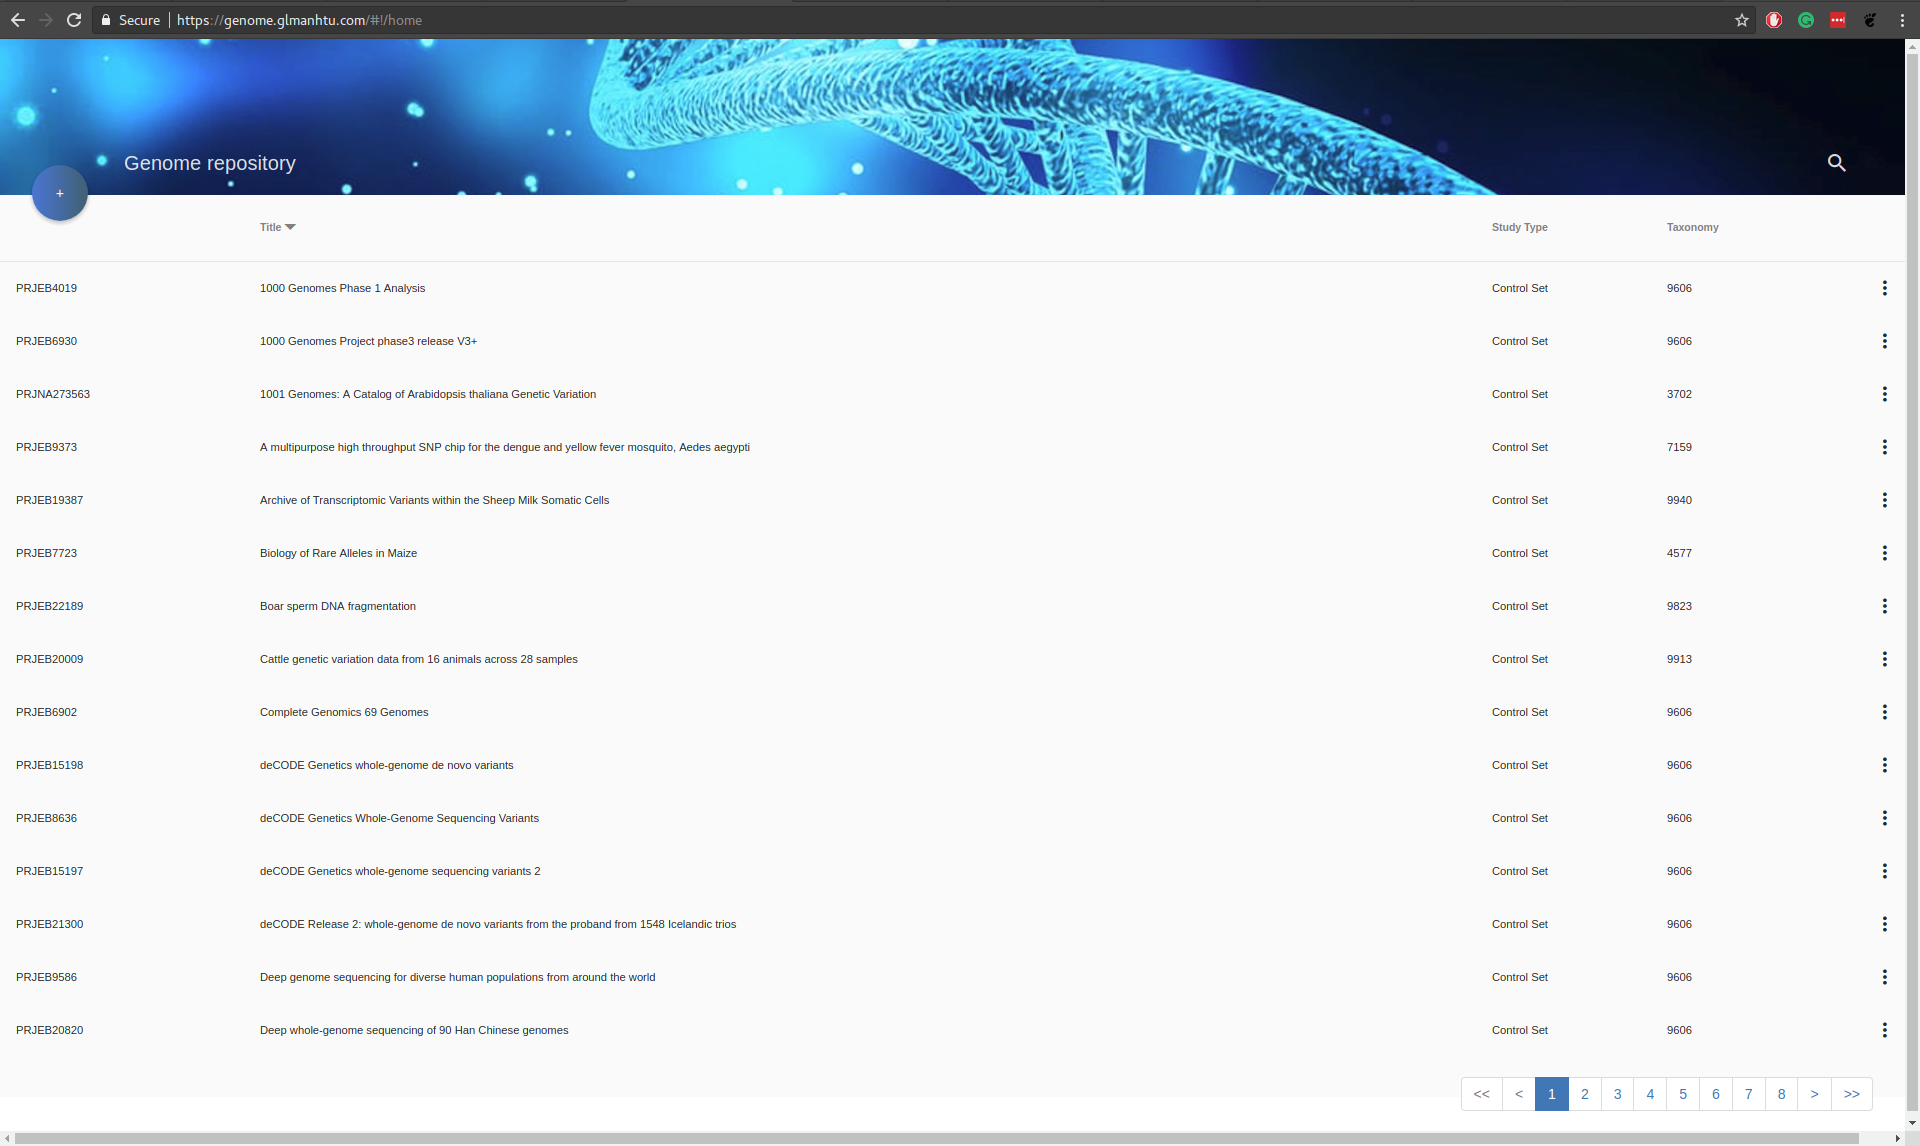
\includegraphics[width=0.99\textwidth]{images/genome-overview}
\caption{Genome application overview}
\end{figure}
\subsection{Find all studies}
The application will list all studies in the home screen and also support sorting and paging projects.
\subsubsection{Sort project studies}
To sort project studies by specific column, simply click to the column header and all results will be sorted as you expected.

\begin{figure}[H]
\centering
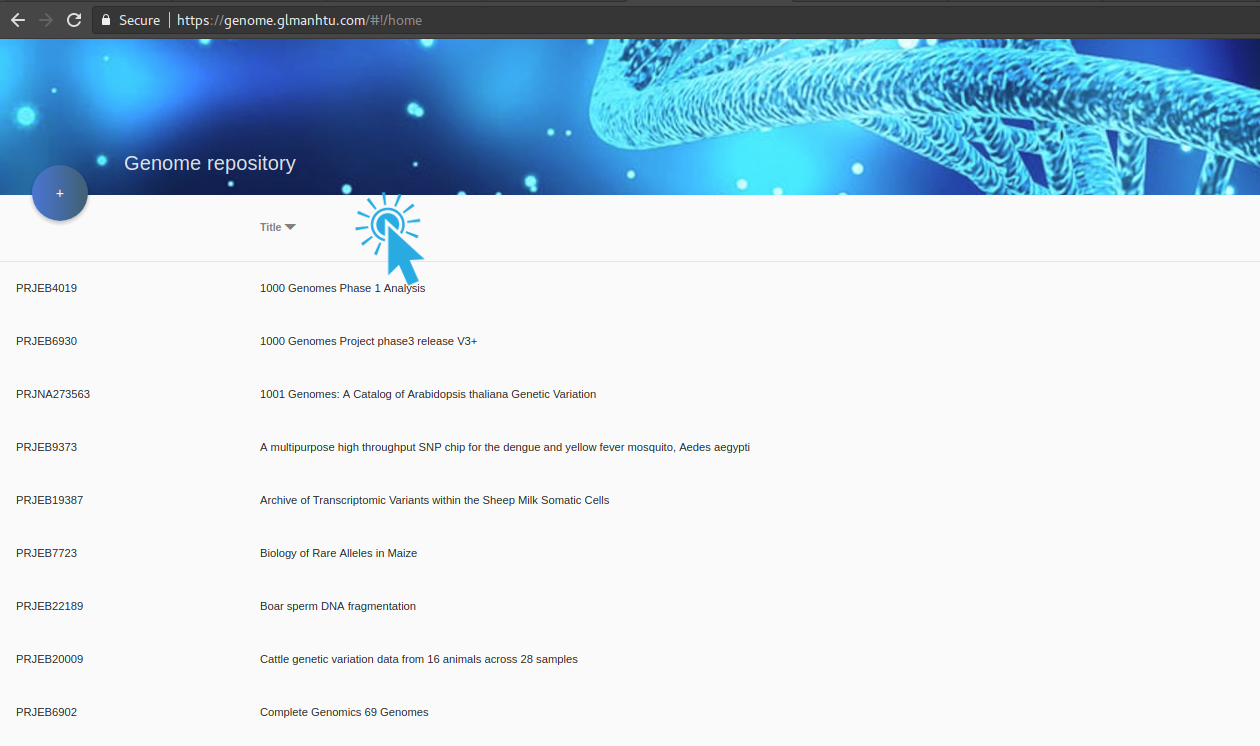
\includegraphics[width=0.99\textwidth]{images/genome-order-2}
\caption{Genome application ordered by title}
\end{figure}

\subsubsection{Paging project studies}
Because we have a lot of project studies, if we call API and get all of them to display, the browser will crash caused by lack of memory/cpu requirement. To avoid this problem, we have implemented the Paging feature. The application will  fetch and display 15 items per page. When the user wants to see more, just change the current page by click the page number button at the end of the result list.

\begin{figure}[H]
\centering
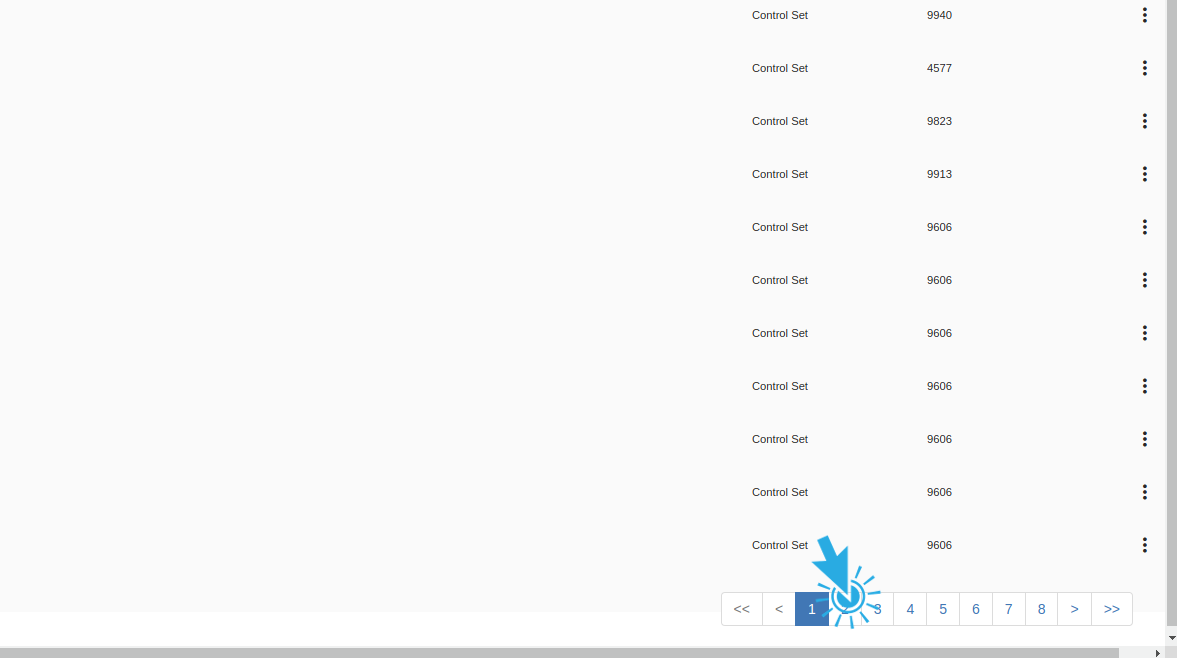
\includegraphics[width=0.99\textwidth]{images/genome-paging}
\caption{Genome application paging}
\end{figure}

\subsection{Filter project studies by taxonomy id}
To filter project studies by \texttt{Taxonomy Id}, just click the search button at the top right of application. Select search by \texttt{Taxonomy Id}, insert the taxonomy id you want to filter to the next input box and press enter.\\
This will filter all project studies, which have its taxonomy id are equals to the keyword.\\
Paging \& Order features also work with this feature.

\begin{figure}[H]
\centering
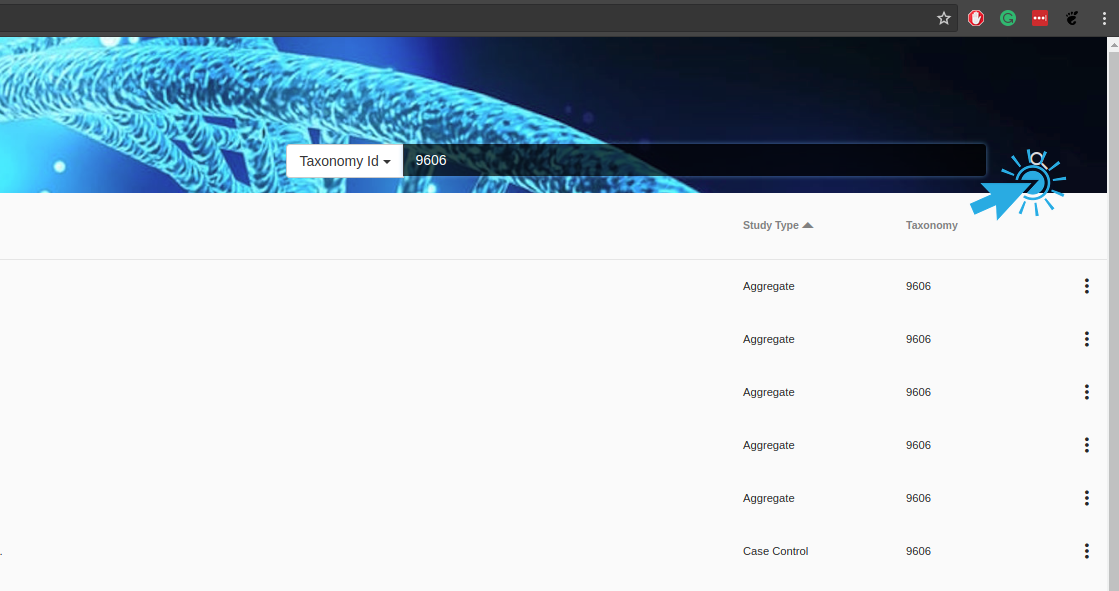
\includegraphics[width=0.99\textwidth]{images/genome-filter-taxonomy}
\caption{Genome application filter by taxonomy id}
\end{figure}

\subsection{Filter project studies by study type}
To filter project studies by \texttt{Study Type}, just click the search button at the top right of application. Select search by \texttt{Study Type}, insert the study type you want to filter to the next input box and press enter.\\
This will filter all project studies, which have study type are containing the keyword.\\
Paging \& Order features also work with this feature.

\begin{figure}[H]
\centering
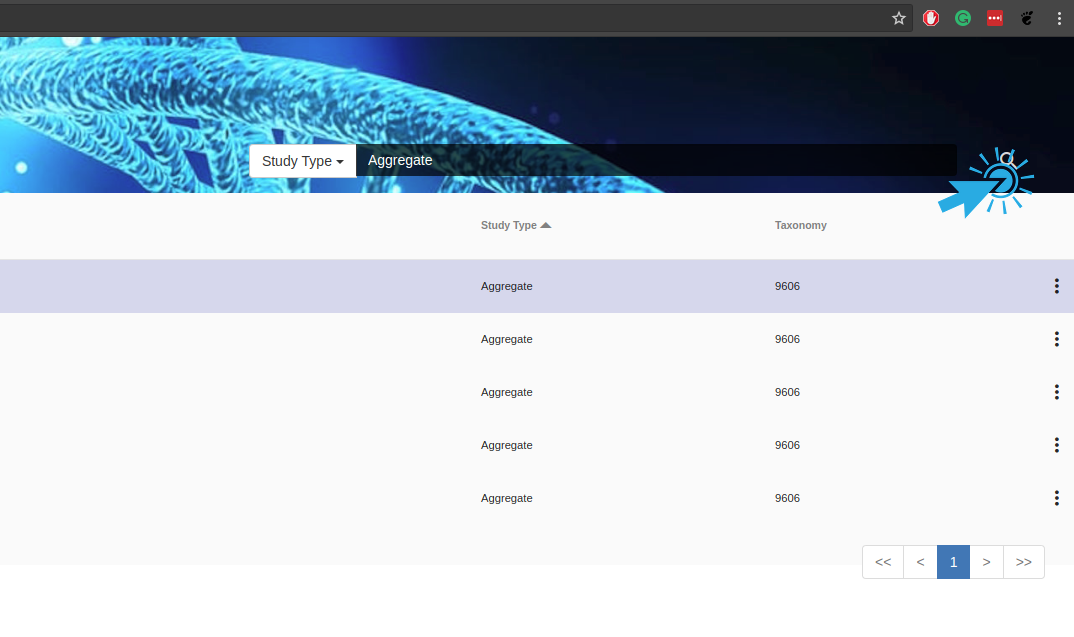
\includegraphics[width=0.99\textwidth]{images/genome-filter-studytype}
\caption{Genome application filter by study type}
\end{figure}

\subsection{Supported the whole set of CRUD operations}
\subsubsection{Create a project study}
To create a project study, click to the add button at the top left of the application. A popup dialog will appear for you to fill the project details form. Once you filled all fields, click \texttt{Create Project} to create. 

\begin{figure}[H]
\centering
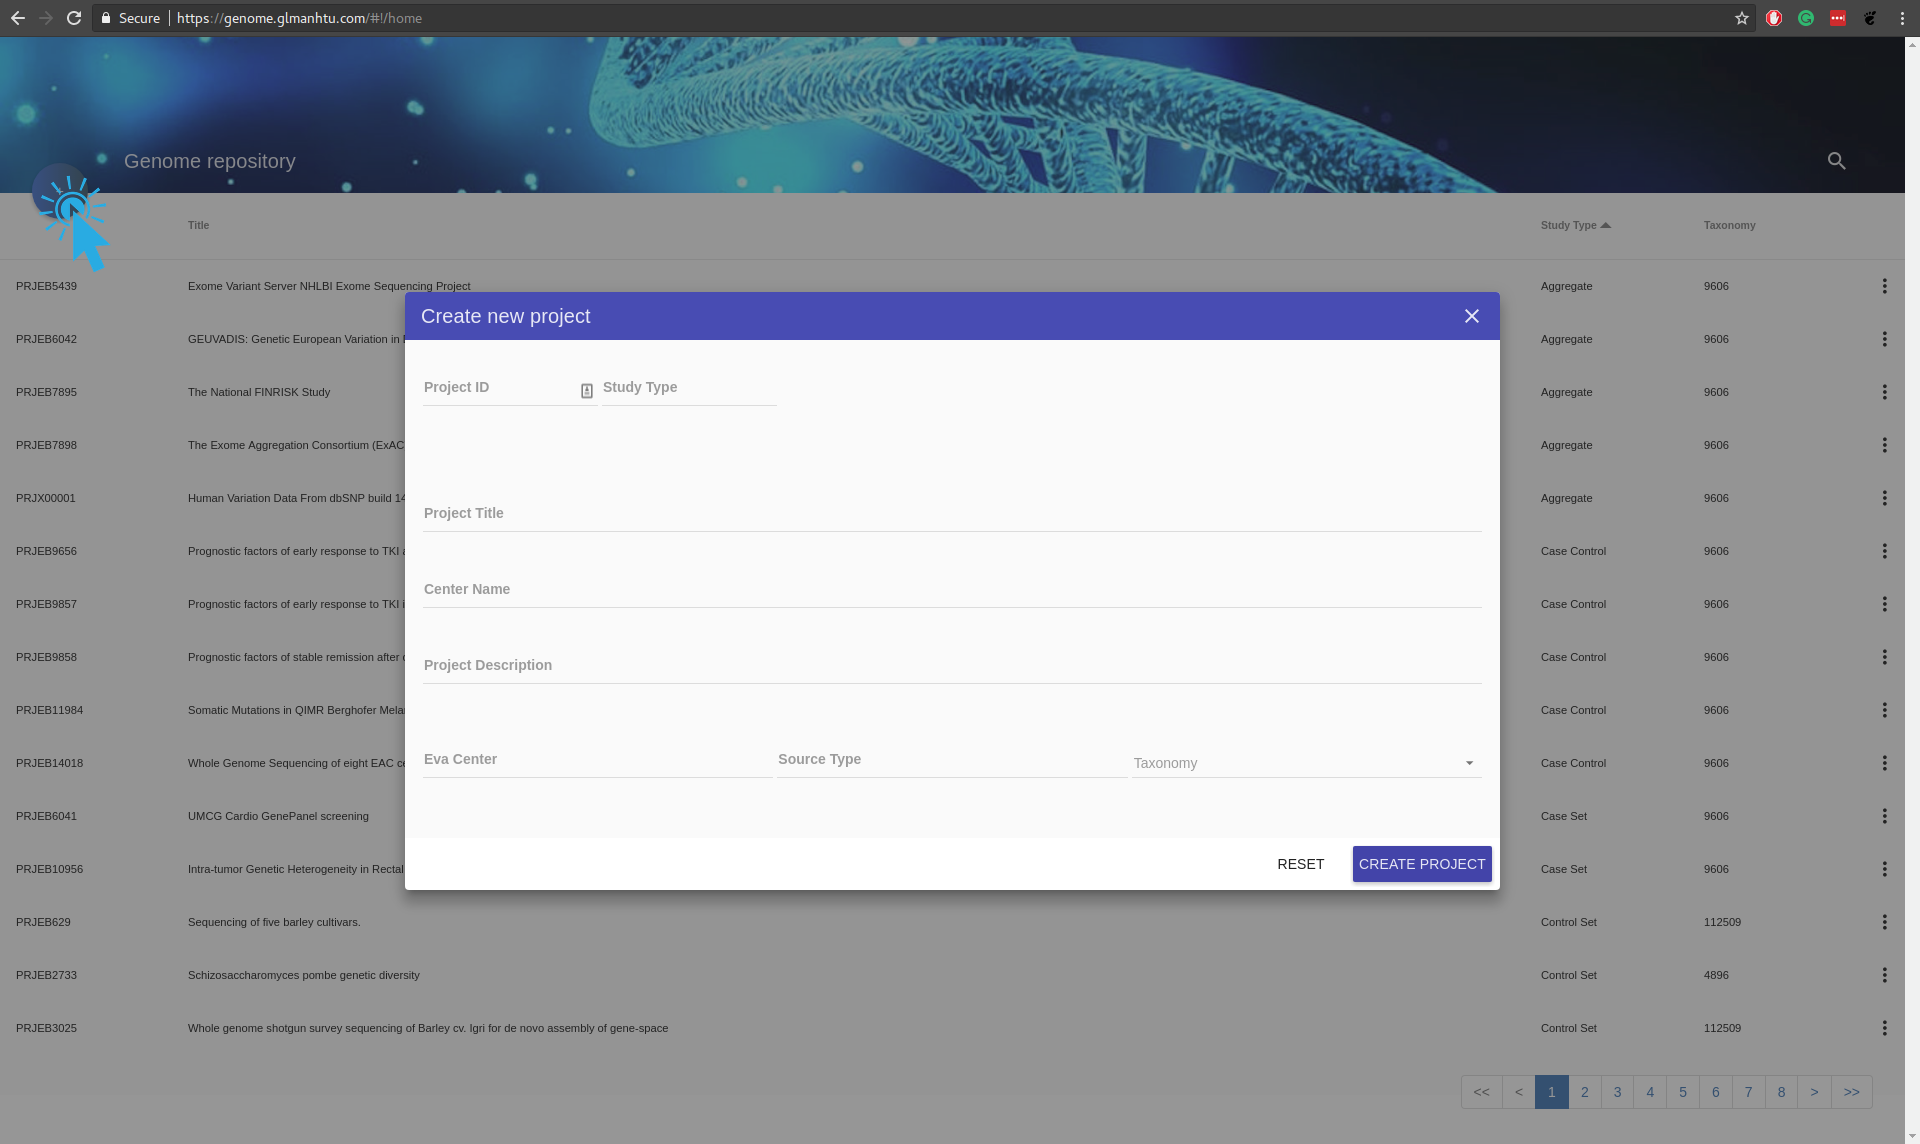
\includegraphics[width=0.99\textwidth]{images/genome-create}
\caption{Genome application create a new project study}
\end{figure}

The notification message will tell you whether your new project study created or not. It also let you know which mistake you made if a problem occurred.

\begin{figure}[H]
\centering
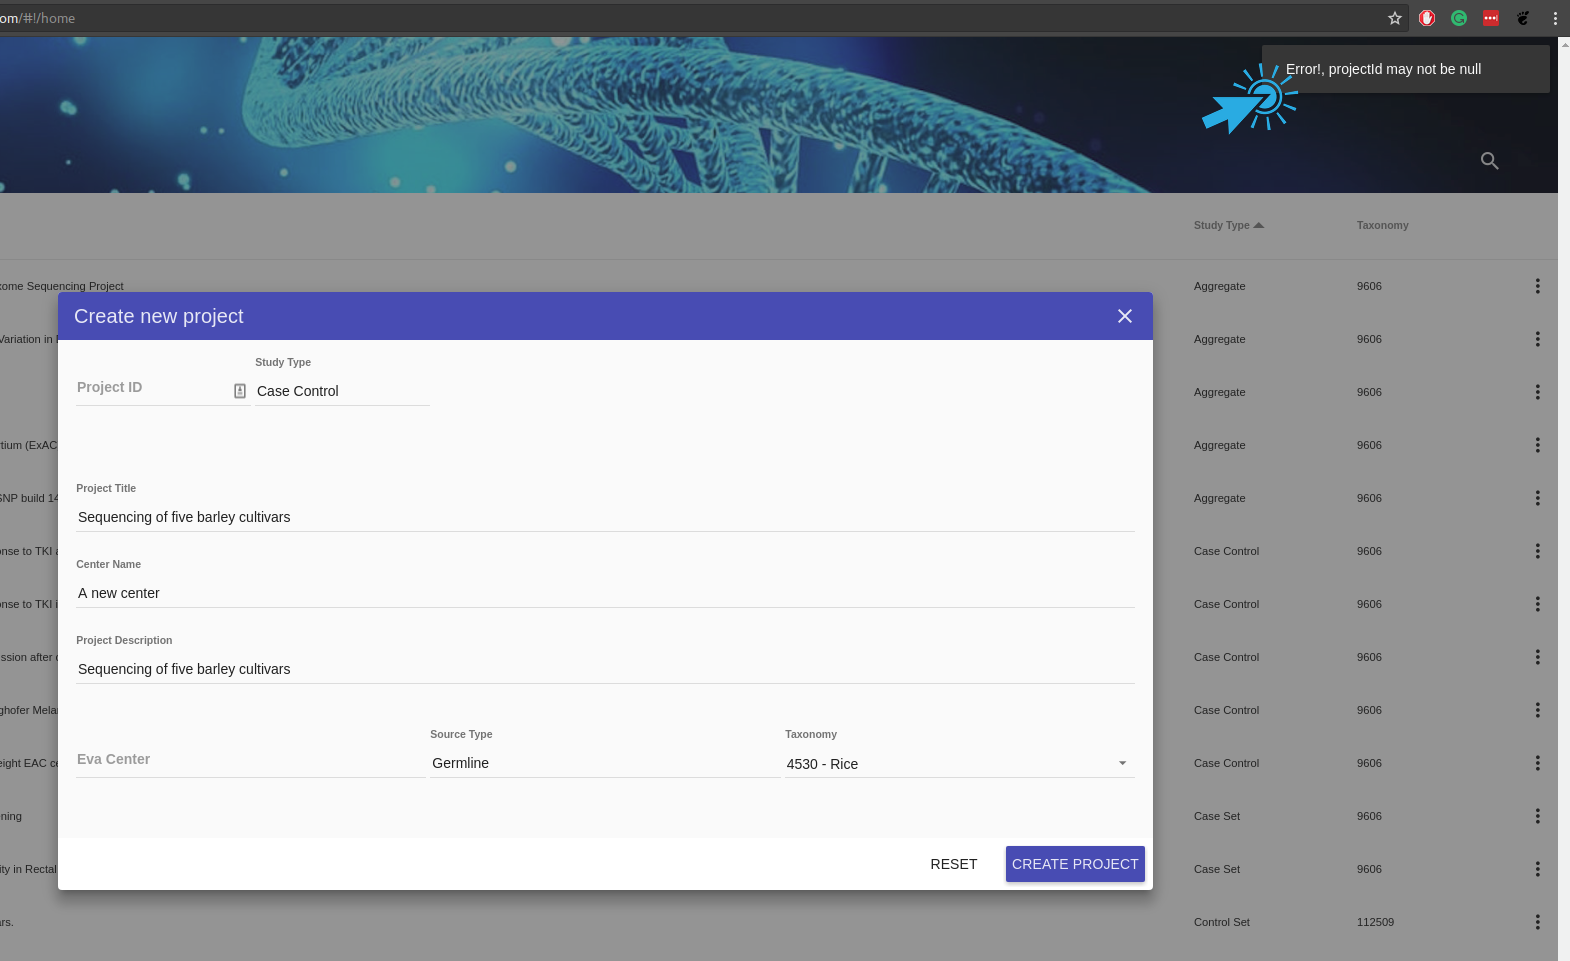
\includegraphics[width=0.99\textwidth]{images/genome-create-notification}
\caption{Genome application notification}
\end{figure}

\subsubsection{Read the details for a single project study}
To view a project study, click on the one you want from the list of project studies. A popup dialog will appear with completed details of the project study.

\begin{figure}[H]
\centering
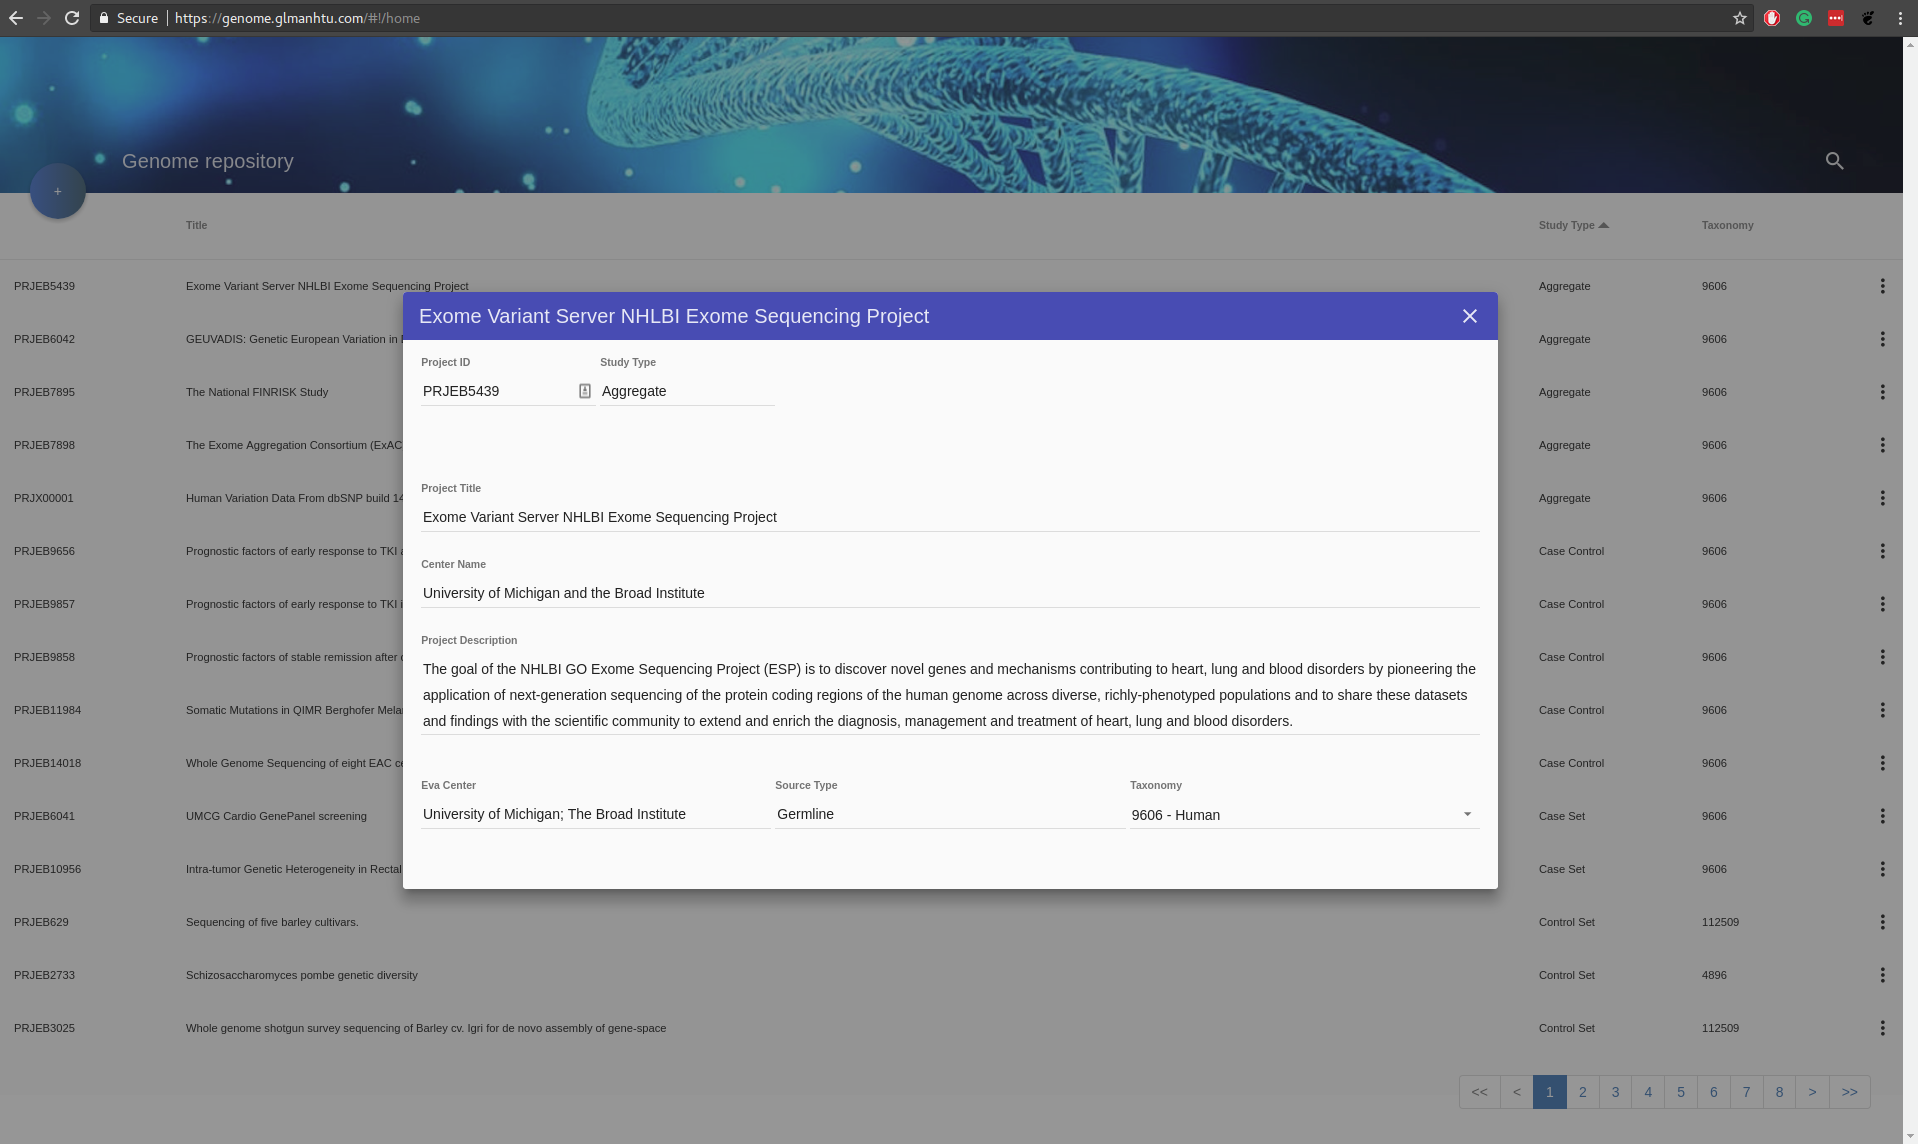
\includegraphics[width=0.99\textwidth]{images/genome-details}
\caption{Genome application details of project study}
\end{figure}

\subsubsection{Update a project study}
To update a project study, click on three-dot-button at the right of the one you want to update and select \texttt{Update Project}. A popup dialog with details of the project study will appear, you can change any fields (except projectId). Finally, click \texttt{Update Project} to update.

\begin{figure}[H]
\centering
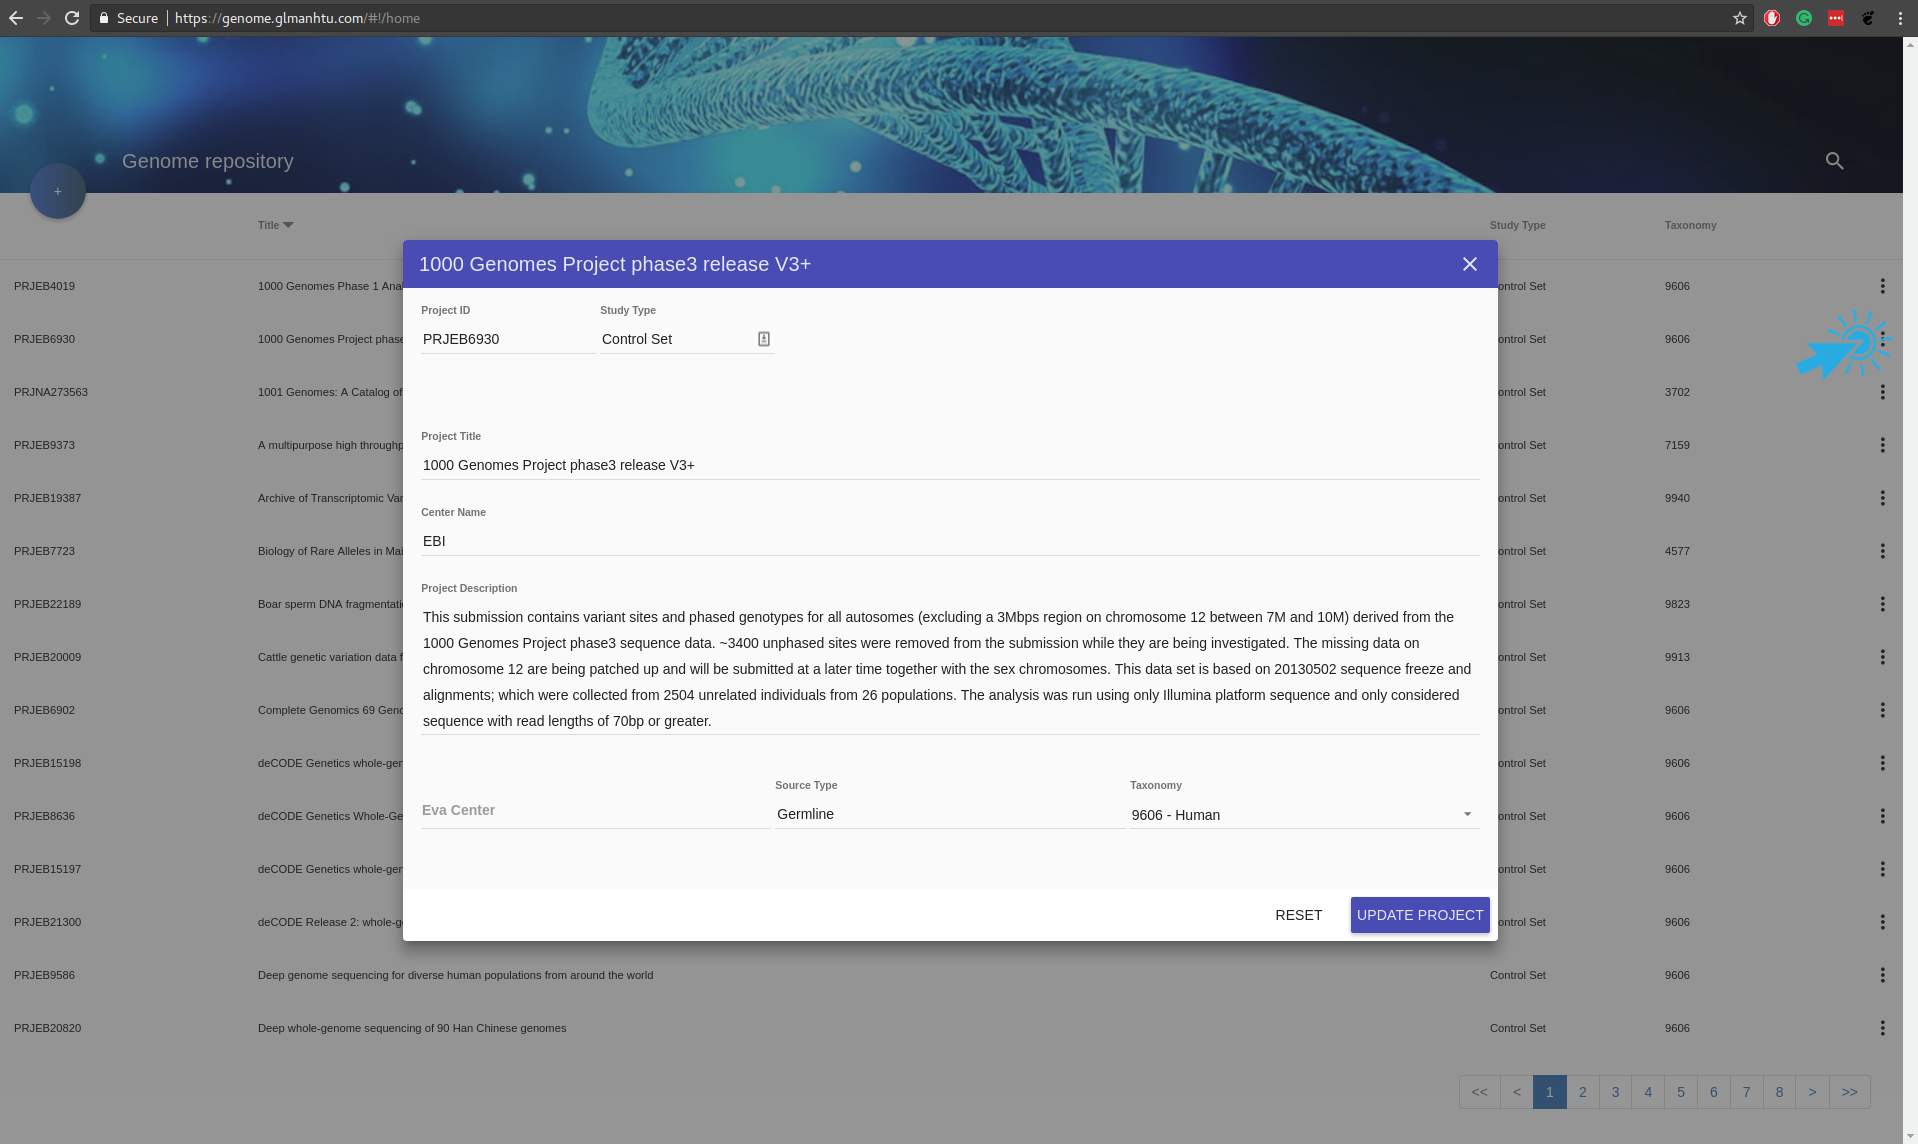
\includegraphics[width=0.99\textwidth]{images/genome-update}
\caption{Genome application update a exist project study}
\end{figure}

\subsubsection{Delete a project study}
To delete a project study, click on three-dot-button at the right of the one you want to update and select \texttt{Delete Project}. A confirm dialog will appear to make sure this isn't an accident. Click \texttt{Please Do It} to delete or \texttt{Maybe another time} to cancel.

\begin{figure}[H]
\centering
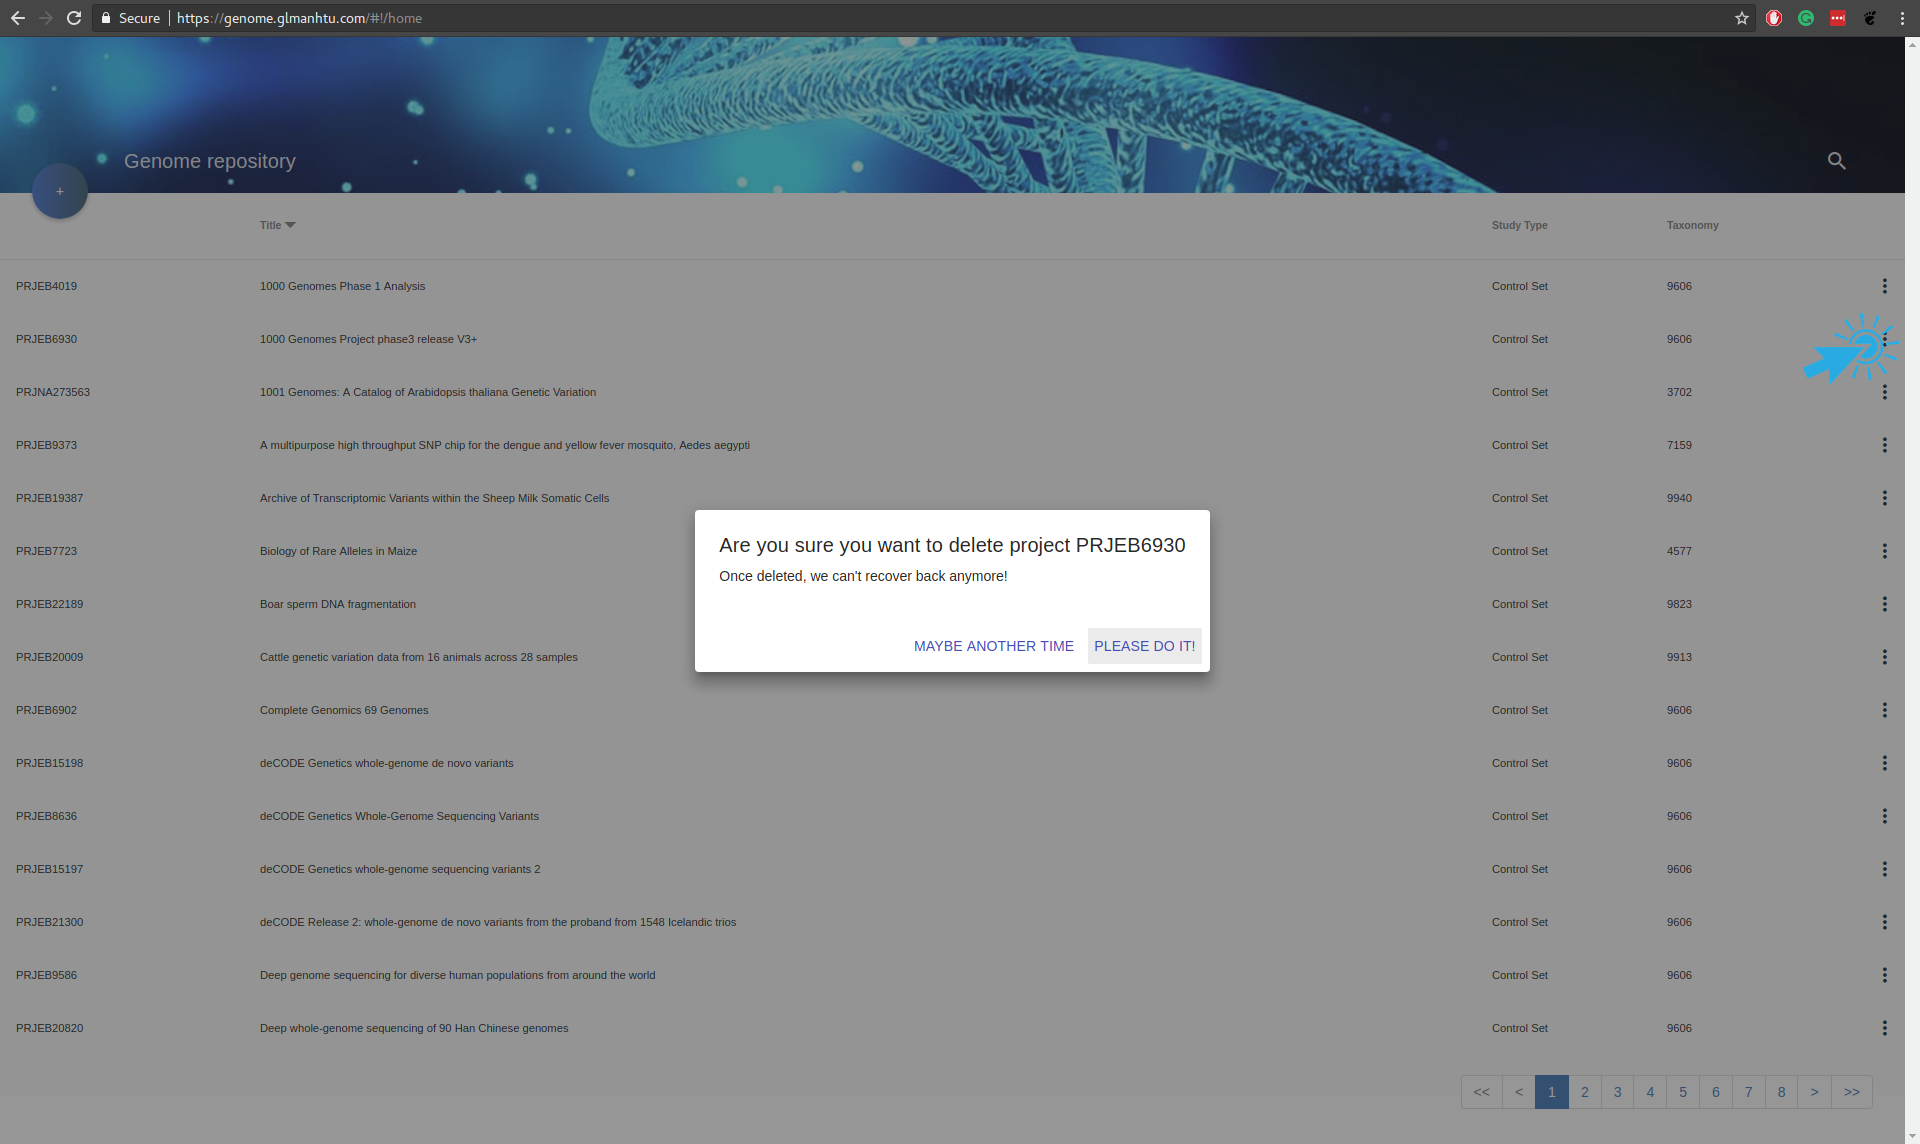
\includegraphics[width=0.99\textwidth]{images/genome-delete}
\caption{Genome application delete a exist project study}
\end{figure}

\subsection{Supporting more filters}
\subsubsection{Filter project studies by title}
To filter project studies by \texttt{Title}, just click the search button at the top right of application. Select search by \texttt{Title}, insert the title you want to filter to the next input box and press enter.\\
This will filter all project studies, which have its title are containing the keyword.\\
Paging \& Order features are also work with this feature.

\begin{figure}[H]
\centering
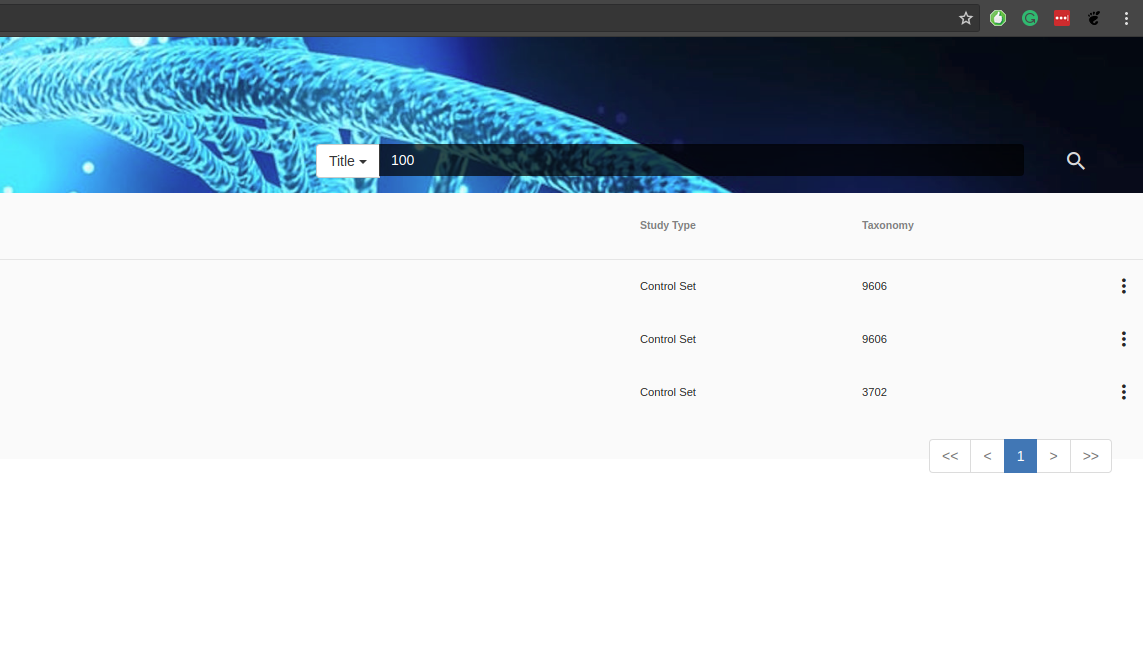
\includegraphics[width=0.99\textwidth]{images/genome-filter-title}
\caption{Genome application filter by title}
\end{figure}
\subsubsection{Filter project studies by project id} 
To filter project studies by \texttt{Project ID}, just click the search button at the top right of application. Select search by \texttt{Project ID}, insert the project id you want to filter to the next input box and press enter.\\
This will filter all project studies, which have its project id are containing the keyword.\\
Paging \& Order features are also work with this feature.

\begin{figure}[H]
\centering
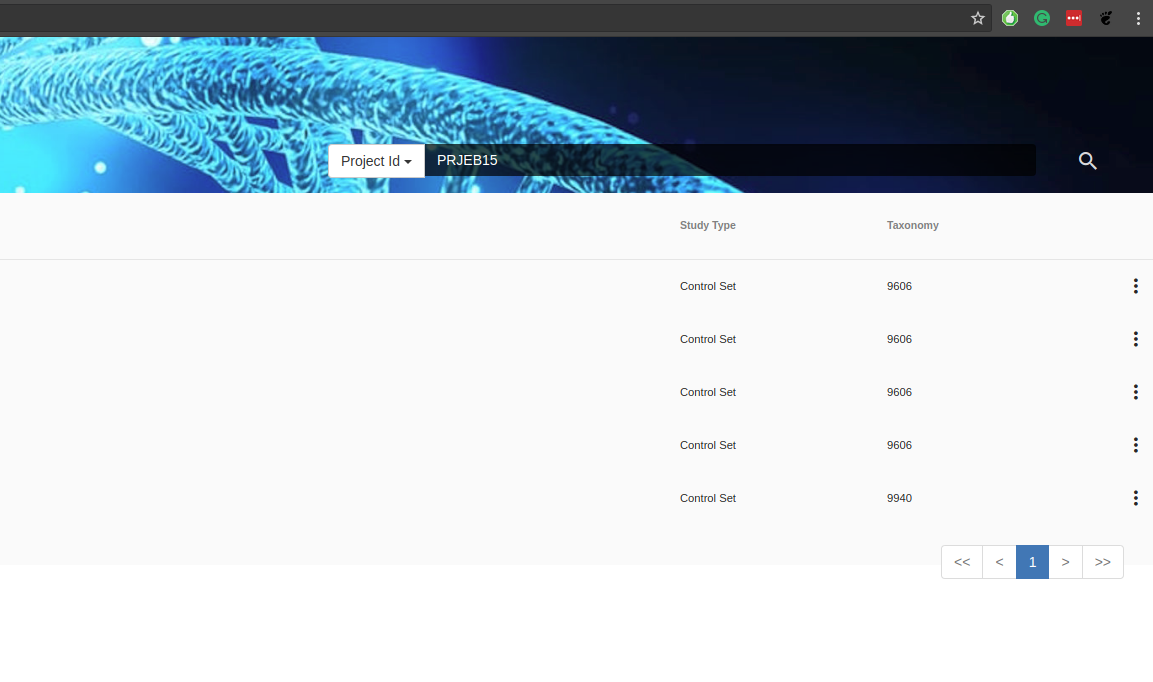
\includegraphics[width=0.99\textwidth]{images/genome-filter-projectid}
\caption{Genome application filter by project id}
\end{figure}


\section{Framework and programming language}
\subsection{The frontend}
AngularJS\footnote{ \url{www.angularjs.org}} is my main framework because:
\begin{itemize}
	\item AngularJS require you to split your app into MVC\footnote{ Model–view–controller} components and then it manages your components for you and also serves as the pipeline that connects them.
	\item Directives achieve this by enabling us to invent our own HTML\footnote{ Hypertext Markup Language} elements. By putting all our DOM\footnote{ Document Object Model} manipulation code into directives, we can separate them out of our MVC app. This allows our MVC app to only concern itself with updating the view with new data.
	\item Filters filter the data before they reach the view and can involve something as simple as formatting decimal places on a number, reversing the order of an array, filtering an array based on a parameter, or implementing pagination. Filters are designed to be standalone functions that are separate from your app, similar to Directives, but are only concerned with data transformations.
	\item All the points up till now mean that you get to write less code. You don’t have to write your own MVC pipeline. The view is defined using HTML, which is more concise. Data models are simpler to write without getters/setters. Data-binding means you don’t have to put data into the view manually. Since directives are separate from app code, they can be written by another team in parallel with minimal integration issues. Filters allow you to manipulate data on the view level without changing your controllers.
	\item Services are exactly what they sound like. They don’t get involved with the MVC of your app, but simply provide an outward API\footnote{ Application programming interface} to expose whatever you want it to expose. Most of the time it syncs up to a server to maintain an offline data store and exposes methods to push and pull data to and from a server. Or it can be used to create a resource sharing service that allows multiple controllers to share the same resources.
	\item Data models in Angular are plain old JavaScript objects and don’t require extraneous getter and setter functions. You can add and change properties directly on it and loop over objects and arrays at will. Your code will look much cleaner and more intuitive, the way mother nature intended.
\end{itemize}
I also applied some technicals to make the development and
control project easier such as NPM\footnote{ \url{https://www.npmjs.com/}} to create a local server, Bower\footnote{ \url{https://bower.io/}} as package control, Gulp\footnote{ \url{https://gulpjs.com/}} as automatic builder tool and SASS\footnote{ \url{http://sass-lang.com/}} to control UI style.

\subsection{API Docs}
You can view and also test my APIs at \url{https://genome.docs.apiary.io}

\subsection{The backend}
I use Java Spring framework and java programming language because:
\begin{itemize}
	\item Java Spring\footnote{ \url{https://spring.io/}} is MVC framework base on JavaEE and compatible a huge library of Java can use in this project without problem. In orther hand, Java Spring has supported from very lage Java Comunication. Which Java Spring framework (Spring Boot) was make easier and automatically to config system that help team save a lot of time and avoid errors.
	\item It is open source and benefit of a large developers community
\end{itemize}

\section{Deployment}
The application have been implemented by both Chef\footnote{ \url{https://www.chef.io/}} and Docker\footnote{ \url{https://www.docker.com/}}.
\subsection{Chef}
With Chef deployment, the developer can deploy your application, install all dependencies and configure your clean new virtual private machine (VPS) with a single command. However, it require to install \& configure Chef workstation. 
\\
\begin{lstlisting}[language=bash]
  $ knife bootstrap <Ip of server> -N '<node name>' -r 'role[<environment>]' --ssh-user <user name on node> --sudo --ssh-identity-file <ssh private credential> --secret-file <location of secret file>
\end{lstlisting}

With `prod` environment, this command will check, install \& configure (if not exist):
\begin{itemize}
	\item \textbf{Oracle\footnote{ \url{https://www.oracle.com}} Java JDK}
	\item \textbf{Git}: clone or pull changes from git repository
	\item \textbf{Maven\footnote{ \url{https://maven.apache.org/}}}: build project
	\item \textbf{Nginx\footnote{ \url{https://www.nginx.com}}}: forward port for backend or web-server for frontend
	\item \textbf{NodeJS\footnote{ \url{https://nodejs.org/}}}: build frontend
\end{itemize}

If your git repository is private, Chef also supports to inject private deploy key and encrypt it via the secret file.
\\\\
Once your VPS bootstrapped, you can easy to re-deploy to get your changes from git repository take effect by one of the following ways:
\\
\\
\indent\textbf{Method 1}: Stay at your workstation and run the following command to re-deploy all your VPS:
\begin{lstlisting}[language=bash]
  $ knife ssh `name:*' `sudo chef-client'
\end{lstlisting}

\textbf{Method 2}: Connect to your VPS and type the following command:
\begin{lstlisting}[language=bash]
  $ sudo chef-client
\end{lstlisting}
\subsection{Docker}
The Docker integration with this application is focus on the end user since it doesn't require to configure anything.
Suppose you already installed docker and docker-compose, you just need to move the terminal console to the source code folder and type the following command:
\begin{lstlisting}[language=bash]
$ docker-compose up
\end{lstlisting}
After the docker-compose booted, you can access the application in your browser at \url{http://127.0.0.1}

\section{Testing}
I have implemented both unit and integration tests to make sure the application work well. Moreover, using those tests allows to address the problems during the development process in an easy way.
\subsection{Unit tests}
The unit tests are located at \texttt{/src/test/java/com/ebi/genome/service/} and independent from the others. You can run those tests using Maven by the following command at the project source root:
\\
\begin{lstlisting}[language=bash]
  $ mvn clean test
\end{lstlisting}

\subsection{Integration tests}
The integration tests are located at \texttt{/src/integration-test/java/com/ebi/genome/} and required you have to specific the database server for this tests. You can do it by modify the \texttt{/src/main/resources/profile/application-integration-test.properties} file as below:

\begin{lstlisting}[language=java]
  spring.datasource.url = jdbc:mysql://<ip>:<port>/<db test>
  spring.datasource.username = <mysql username>
  spring.datasource.password = <mysql password>

  # Keep the connection alive if idle for a long time (needed in production)
  spring.datasource.testWhileIdle = true
  spring.datasource.validationQuery = SELECT 1
\end{lstlisting}
However, in the source code, I already updated those parameters by my running database (Google Cloud SQL) details. So, you can try to test with it.
\\
\\
To run the integration tests, execute the following command at the source root:
\\
\begin{lstlisting}[language=bash]
  $ mvn clean verify
\end{lstlisting}
\section{Known problems and limitation}
\subsection{Mobile display problem}
Currently, the application works well on the desktop but not on mobile device. You still can open the website in your mobile's browser but the style displayed isn't good.
\subsection{Fixed columns to display on list of projects}
Currently, the application fixed display four columns because of not enough space to display. Those columns include project id, title, study type and taxonomy. However, a better solution could let the user choose what column they want to display. This feature could be implement in the future.
\subsection{Unsupported combine search}
The application supports multi kind of searches such as project id, title, study type or taxonomy id. However, it could be nice if we can combine multiple search type at one time. It's possible if we are using Spring Data JPA Specification. However, because of lacking time, this feature could be implemented in the future.
\end{document}